\documentclass[12pt]{article}
%packages
\usepackage[top=1in, bottom=1in, left=.75in, right=.75in]{geometry}
\usepackage{amsmath, enumerate}
\usepackage{fancyhdr}
\usepackage{graphicx, xcolor, setspace, array}
\usepackage{txfonts}
\usepackage{multicol,coordsys,pgfplots}
\usepackage[scaled=0.86]{helvet}
\usepackage{anyfontsize}
\usepackage{tikz,pgfplots}
\usetikzlibrary{calc,arrows.meta}

% specials
\renewcommand{\emph}[1]{\textsf{\textbf{#1}}}
\def\ra{\rightarrow}
\pgfplotsset{compat = newest}
\newcommand{\blank}[1]{\rule{#1}{0.75pt}}
\pgfplotsset{my style/.append style={axis x line=middle, axis y line=
middle, xlabel={$x$}, ylabel={$y$}}}
\newcommand{\be}{\begin{enumerate}}
\newcommand{\ee}{\end{enumerate}}
\newcommand{\ans}[1][1in]{\rule{#1}{.5pt}}
\newcommand{\ul}[1]{\underline{#1}}
\let\ds\displaystyle
\def\continued{{\emph {Continued....}}}
\def\continuing{{\emph {Problem \arabic{probcount} continued....}}\par\vskip 4pt}

%page setup
\parindent 0pt
\parskip 4pt
\pagestyle{fancy}
\fancyfoot[C]{\emph{\thepage}}
\fancyfoot[R]{} %%%%%% <-- Version Info
\fancyhead[L]{\ifnum \value{page} > 1\relax\emph{Math F113X: Exam 1}\fi}
\fancyhead[R]{\ifnum \value{page} > 1\relax\emph{Spring 2026}\fi}
\headheight 15pt
\renewcommand{\headrulewidth}{0pt}
\renewcommand{\footrulewidth}{0pt}

% Problem Set up 
%% REALLY?
\newcounter{probcount}
\newcounter{subprobcount}
\newcommand{\thesubproblem}{\emph{\alph{subprobcount}.}}
\def\problem#1{\setcounter{subprobcount}{0}%
\addtocounter{probcount}{1}{\emph{\arabic{probcount}.\hskip 1em(#1)}}\par}
\def\subproblem#1{\par\hangindent=1em\hangafter=0{%
\addtocounter{subprobcount}{1}\thesubproblem\emph{#1}\hskip 1em}}
\def\probskip{\vskip 10pt}
\def\medprobskip{\vskip 2in}
\def\subprobskip{\vskip 45pt}
\def\bigprobskip{\vskip 4in}
\newenvironment{subproblems}{%
\begin{enumerate}%
\setcounter{enumi}{\value{subprobcount}}%
\renewcommand{\theenumi}{\emph{\alph{enumi}}}}%
{\setcounter{subprobcount}{\value{enumi}}\end{enumerate}}

%%%%%
% Document Begins
\begin{document}

{\emph{\fontsize{26}{28}\selectfont Spring 2026 \hfill
\hfill Math F113X}}

\begin{center}
{\emph{
{\fontsize{32}{36}\selectfont Exam 1}}
}
\end{center}

\vfill
\emph{\fontsize{18}{22}\selectfont Name:\underline{\hspace{2in}}\hspace{2cm} Instructor: \underline{\hspace{2in}}}\\


\vfill
{\fontsize{18}{22}\selectfont\emph{Rules:}}

\begin{itemize}
\item Partial credit will be awarded, but you must show your work.

\item You may have a $3 \text{in} \times 5 \text{in} $ notecard with writing on both sides.

\item Calculators are allowed. 

\item Turn off anything that might go beep during the exam.

\end{itemize}




Good luck!

\vfill
\def\emptybox{\hbox to 2em{\vrule height 16pt depth 8pt width 0pt\hfil}}
\def\tline{\noalign{\hrule}}
\centerline{\vbox{\offinterlineskip
{
\bf\sf\fontsize{18pt}{22pt}\selectfont
\hrule
\halign{
\vrule#&\strut\quad\hfil#\hfil\quad&\vrule#&\quad\hfil#\hfil\quad
&\vrule#&\quad\hfil#\hfil\quad&\vrule#\cr
height 3pt&\omit&&\omit&&\omit&\cr
&Problem&&Possible&&Score&\cr\tline
height 3pt&\omit&&\omit&&\omit&\cr
&1&&16 &&\emptybox&\cr\tline
&2&&8	&&\emptybox&\cr\tline
&3&&10	&&\emptybox&\cr\tline
&4&&10	&&\emptybox&\cr\tline
&5&&12	&&\emptybox&\cr\tline
&6&&12	&&\emptybox&\cr\tline
&7&&10	&&\emptybox&\cr\tline
&8&&12	&&\emptybox&\cr\tline
&9&&10	&&\emptybox&\cr\tline
&Extra Credit&&(4)&&\emptybox&\cr\tline
&Total&&100&&\emptybox&\cr
}\hrule}}}

\newpage

\begin{enumerate}
%% General + IRV
\item (16 pts.~total) \label{prob:jr-one} Consider the following preference schedule for an election with 4 candidates and 100 voters.

\begin{center}
\begin{tabular}{c||c|c|c|c|c|}
&24&10&21&27&18\\
\hline\hline
1st&A&B&D&C&B\\
2nd&C&A&A&D&A\\
3rd&D&C&C&A&C\\
4th&B&D&B&B&D
\end{tabular}
\end{center}

	\begin{enumerate}

	\item  (3 pts.) Who wins a plurality vote in this election? Show your work.
\vfill

%	\item (3 pts.) If opinion polls before the election showed A was running behind several other candidates, the voters ranking A first might have decided to instead vote for their second choice in this plurality election. What is the name for this type of voting behavior?
%\vfill
%	\item (3 pts.) If opinion polls before the election showed A was running behind several other candidates, the voters ranking A first might have decided to instead vote for their second choice. Would this action  have changed the outcome? Who would have won? 
%\vfill



	\item (8 pts.) If instead an IRV (ranked choice) election was held, the first round would not produce a winner, but D would be eliminated. Knowing this, determine the outcome of the {\bf second round}, showing your work. Give the winner (if there is one), or say who is eliminated next.
\vfill

\vfill

\hspace*{-.2in}Candidate who wins in second round:\underline{\ \ \ \ \ \ \ \ \ }
\ \ \ \ \ OR Candidate eliminated after second round:\underline{\ \ \ \ \ \ \ \ \ }\\


\item (5 pts.) If opinion polls before the election showed A was running behind several other candidates, the voters ranking A first might have decided to instead vote for their second choice. Would this action  have changed the outcome? Who would have won? 
\vfill
	\end{enumerate}


\newpage

%%% Borda
\item (8 pts.) 

\begin{minipage}{4.in} A Borda Count will be used to determine the winner in the election with voting schedule on the right. 
\end{minipage}
\hskip.3in
\begin{tabular}{c||c|c|c}
&2&5&7\\
\hline\hline
1st&A&B&C\\
2nd&C&C&B\\
3rd&B&A&A
\end{tabular}

	\begin{enumerate}
	\item (4 pts) Showing your work, calculate the weighted vote for candidate B.
	
	\vfill
	
	\item (2 pts) If the weighted vote for candidate A is 18 and for candidate C is 35, who is the Borda winner?
	\vspace{.2in}
	\item (2 pts) Is the Borda winner also a majority winner? Explain you reasoning.
	\vspace{.5in}
	\end{enumerate}
	

\item (10 pts.~total)  

\begin{minipage}{4.5in}  In deciding among four candidates for promotion, Abby (A), Burt (B), Camile (C), and David (D), six members of the senior management rank their preferences as shown, and then compile the following table of outcomes from most of the head-to-head match-ups.
\end{minipage}
\hskip .5in
\begin{tabular}{c||c|c|c}
&2&1&3\\
\hline\hline
1st&A&B&C\\
2nd&B&C&A\\
3rd&C&D&B\\
4th&D&A&D\\
\end{tabular}



\begin{center}
\begin{tabular}{c||c|c|c|c|c|c|}
Match up&A vs. B&A vs. C&A vs. D&B vs. C&B vs. D&C vs. D\\
\hline\hline
Winner&A&  &A&tie&B&C
\end{tabular}
\end{center}


	\begin{enumerate}

	\item(3 pts.) Who would win the A vs.~C head-to-head vote? Show your work.
\vfill

	\item (3 pts.) Is there a Condorcet winner? Explain why or why not.
\vfill
	\item  (4 pts.) Who would win by Copeland's method? Show work to support your answer.
	\vfill
	\end{enumerate}


\newpage
%%Basic Weighted Voting
\item (10 pts) Consider the weighted voting system $[18: 8,4,4,3,3,2]$. Find:

	\begin{enumerate}
	\item (2 pts) The total number of players: \vspace{0.4in}

	\item (2 pts) The total number of votes: \vspace{0.4in}

	\item (2 pts) The quota: \vspace{0.4in}

	\item (4 pts) Identify which players have veto power. Show a calculation that justifies your conclusion.
	\vspace{1in}
	\end{enumerate}

\item (12 pts)  Consider the weighted voting system $[q: 9, 4, 2]$.

	\begin{enumerate}
	\item (3 pts) What is the smallest possible quota value? \vspace{0.5in}

	\item (4 pts) Find \emph{all} possible values of $q$ that result in a dictator.  \emph{State which player} is the dictator and \emph{explain} why this is the case. \vfill
	\item (5 pts) Find \emph{all} possible values of $q$ that result in one or more dummies? \emph{State which player(s)} are dummies and \emph{explain} why this is the case. \vfill \vfill	\end{enumerate}

\newpage
%% Banzhaf
\item (12 pts) Consider the weighted voting system $[29: 17, 13, 12, 4]$. A list of all seven \emph{winning} coalitions are listed below. The critical players have been underlined in each winning coalition \emph{except for the two in boxes.}\\


\begingroup
{\setlength{\fboxsep}{.3cm}
\setlength{\tabcolsep}{10pt} % Default value: 6pt
\renewcommand{\arraystretch}{1.5} % Default value: 1
\begin{tabular}{p{1in}   p{1in} p{1in}  p{1in}}
\multicolumn{4}{c}{All Winning Coalitions}\\
&&&\\
$\ul{P_1}, \, \ul{P_2}$ & $\ul{P_1}, \, P_2,\, P_3$ & $\ul{P_2}, \, \ul{P_3},\, \ul{P_4}$&\fbox{$P_1, \, P_2,\, P_3, \, P_4$}\\
$\ul{P_1}, \,\ul{P_3}$ &  $\ul{P_1}, \, \ul{P_2},\, P_4$  &\fbox{$P_1, \, P_3,\, P_4$} &\\

\end{tabular}
}
\endgroup



	\be
	\item (3 pts) Provide a calculation with explanation demonstrating that the coalition $P_1, P_3, P_4$ is a winning coalition.

\vspace{1.5in}

	\item (4 pts) \emph{For the two winning coalitions in boxes,} underline any players that are critical.  Explain your reasoning below. 	
	\vfill

	\item (5 pts) Find the Banzhaf power distribution for this system. Give each player's power as a fraction.\\
	
	\vspace{.15in}
	\begin{tabular}{| c || >{\centering\arraybackslash}p{1in} | >{\centering\arraybackslash}p{1in} | >{\centering\arraybackslash}p{1in} | >{\centering\arraybackslash}p{1in} |}
	\hline
	player & $P_1$ & $P_2$ & $P_3$ & $P_4$ \\
	\hline
	Banzhaf&&&&\\
	Power &&&&\\
	Index &&&&\\
	\hline
	\end{tabular}


	\ee

\vspace{1in}



\newpage

%% Divider-Chooser
\item(10 pts) Tim and Harold decide to split a pizza with three separate toppings using the {\bf Divider-Chooser} method. The total cost of the pizza is \$32. Below is a picture of the pizza and pictures indicating how Tim and Harold value the parts of the pizza.
%% picture
\begin{multicols}{3}
%% general pizza
\begin{center}
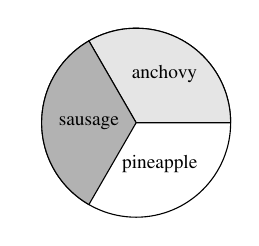
\begin{tikzpicture}[scale=0.6]
\def\r{2}
\draw (0,0) circle (\r cm);
\filldraw[fill= gray!20 ] (0,0) -- (0:\r) arc (0:120:\r) -- (0,0);
\path (60:1.2) node[]{{{\scriptsize anchovy}}};
%\path node[right] (240:1) {{\scriptsize Strawberry}};
\filldraw[fill = gray!60 ] (0,0) -- (120:\r) arc (120:240:\r) -- (0,0);
\path (120+60:\r/2) node[]{{{\scriptsize sausage}}};
\path (-60:\r/2) node[]{{{\scriptsize pineapple}}};
\end{tikzpicture}
\end{center}
%% Tim's
\begin{center}
  Tim
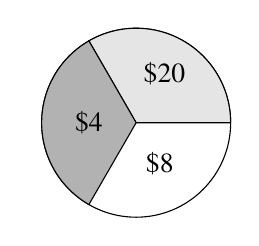
\begin{tikzpicture}[scale=0.6]
\def\r{2}
\draw (0,0) circle (\r cm);
\filldraw[fill= gray!20 ] (0,0) -- (0:\r) arc (0:120:\r) -- (0,0);
\path (60:1.2) node[]{{{\$20}}};
%\path node[right] (240:1) {{\scriptsize Strawberry}};
\filldraw[fill = gray!60 ] (0,0) -- (120:\r) arc (120:240:\r) -- (0,0);
\path (120+60:\r/2) node[]{{{\$4}}};
\path (-60:\r/2) node[]{{{\$8}}};
\end{tikzpicture}
\end{center}
%% Harold's 
\begin{center}
  Harold
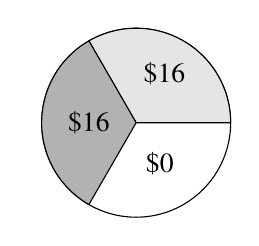
\begin{tikzpicture}[scale=0.6]
\def\r{2}
\draw (0,0) circle (\r cm);
\filldraw[fill= gray!20 ] (0,0) -- (0:\r) arc (0:120:\r) -- (0,0);
\path (60:1.2) node[]{{{\$16}}};
\filldraw[fill = gray!60 ] (0,0) -- (120:\r) arc (120:240:\r) -- (0,0);
\path (120+60:\r/2) node[]{{{\$16}}};
\path (-60:\r/2) node[]{{{\$0}}};
\end{tikzpicture}
\end{center}
\end{multicols}
	% Subproblems Start
	\begin{enumerate}
	\item (2 pts) How much value is a fair share of the pizza? \$ \underline{\hspace{3cm}}
	\item Tim is selected to be the divider and splits the pizza into two shares indicated below in a picture and a table.

\vspace*{-.2in}
\begin{multicols}{2}	
\quad \\
	\begin{tabular}{l || l}
	Share 1:&  all of the sausage, \\ &1/2 of the anchovy, \\&  1/4 of the pineapple\\
	\hline
	Share 2 :&  1/2 of the anchovy,\\& 3/4 of the pineapple\\
	\end{tabular}
	
\vspace*{-.1in}
\begin{center}
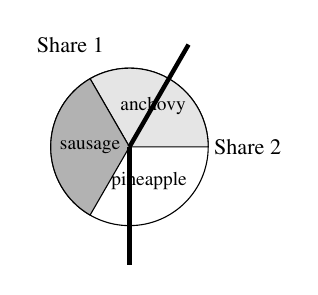
\begin{tikzpicture}[scale=0.5]
\def\r{2}
\draw (0,0) circle (\r cm);
\filldraw[fill= gray!20 ] (0,0) -- (0:\r) arc (0:120:\r) -- (0,0);
\path (60:1.2) node[]{{{\scriptsize anchovy}}};
\filldraw[fill = gray!60 ] (0,0) -- (120:\r) arc (120:240:\r) -- (0,0);
\path (120+60:\r/2) node[]{{{\scriptsize sausage}}};
\path (-60:\r/2) node[]{{{\scriptsize pineapple}}};
\filldraw[ultra thick] (0,0) -- (60:3);
\filldraw[ultra thick]  (0,0) -- (270:3);
\path (0:3) node[]{{{\footnotesize Share 2}}};
\path (120:3) node[]{{{\footnotesize Share 1}}};
\end{tikzpicture}
\end{center}

\end{multicols}
\vspace{-0.5cm}

		%sub-sub problems start
		\be
		\item (4 pts) Provide a calculation that demonstrates Share 2 is a fair share to Tim. \\
		\vfill
		\item (4 pts) Which share would Harold choose? Circle the correct
  answer and provide a calculation to support your answer.
  \begin{center}
    {\bf Share 1} \hspace{5cm} {\bf Share 2}
  \end{center}

\vfill
%		\item (2 pts) Find a \emph{different} division of the pizza into two fair shares based on Tim's values. \\ 
%
%\hspace*{-1cm} Share 1:  \underline{\hspace{2cm}} of the sausage,
%\underline{\hspace{2cm}} of the anchovy,  \underline{\hspace{2cm}}
%of the pineapple  \\
%\vspace{0.5cm}
%  
%\hspace*{-0.9cm}Share 2:  \underline{\hspace{2cm}} of the sausage,
%\underline{\hspace{2cm}} of the anchovy, \underline{\hspace{2cm}}
%of the pineapple \\

		\ee
		%sub-subproblems end
%	\item (2 pts)  In {\bf Divider-Chooser}, why is it better to be the Chooser?
%	\vfill
  
	\end{enumerate}
	%subproblems end
% end Divider-Chooser

\newpage

% Lone Divider
\item (12 pts) Tim, Harold, and Janet will split several bags of coffee worth \$90 using the {\bf Lone Divider} method. One of the three friends is selected to divide the
coffee into three shares. The values are shown
below.

\begin{center}
\begin{tabular}{l|| l| l| l| l}
Person & Share 1 & Share 2 & Share 3 \\ \hline
Tim & \$40 & \$20 & \$30 \\
Harold & \$30 & \$30 & \$30 \\
Janet & \$60 & \$15 & \$15 
\end{tabular}
\end{center}
	%subproblems start
	\begin{enumerate}
	\item (2 pts) What is the value of a fair share to each person?
	\vfill
	\item (3 pts) Who was the divider? How can you tell?
	\vfill
	\item (2 pts) \emph{Circle the bids (dollar values) in the table} that are fair shares to each person.\\
	
	\item (5 pts) Is it possible to allocate the shares so that everyone gets a fair
  share? If so, who gets which share? If not, what happens next in the
  lone divider process?
  \vfill
	\end{enumerate}
	%subproblems end
% End Lone Divider	

\newpage

% begin sealed bids
\item (10 pts) Yelena and Zach are going to divide their shared kitchen gadgets, a coffee maker and a microwave, using the method of sealed bids.  Fill in the blanks below. 
\begingroup

%\setlength{\tabcolsep}{10pt} % Default value: 6pt
\renewcommand{\arraystretch}{1.5} % Default value: 1
\begin{tabular}{|p{3in} || >{\centering\arraybackslash}m{1.5in} |>{\centering\arraybackslash}m{1.5in} |}
\hline
& Yelena & Zach \\ \hline \hline
coffee maker & \$100 & \$90 \\ \hline
microwave & \$50 & \$70 \\ \hline
total bid & \$150 & \$160 \\ \hline
\textbf{(a) (2 pts) What is a \textbf{fair share} for each person?}& & \\ \hline
 award (who gets what item)&coffee maker& microwave \\ \hline
 {award value}& \$ 100 &  \$ 70 \\ \hline
 \textbf{(b) (4 pts)  How much money does each person pay in or receive from the holding pile?} &&  \\
 Make sure to indicate whether the person pays in or receives.&&\\  \hline
 \textbf{(c) (2 pts) Determine the surplus.} &\multicolumn{2}{c|}{\quad} \\[12 pt] \hline
 \textbf{(d) (2 pts) Determine each person's fair share of the  surplus.} &&\\[12 pt] \hline
\end{tabular}

\vfill

\textbf{Extra Credit:} (4 pts) Determine the Final Allocation by filling out each blank below.\\


\renewcommand{\arraystretch}{2} 
\begin{tabular}{ | l || >{\centering\arraybackslash}p{4cm}| >{\centering\arraybackslash}p{4cm} |>{\centering\arraybackslash}p{4cm} |}
\hline
\multicolumn{4}{| c |}{Summary of Final Allocation}\\
\hline
person& items & cash & paid or received? \\

\hline

Yelena&&&\\

\hline

Zach &&&\\
\hline
\end{tabular}

\endgroup
\vfill
\end{enumerate}

%\newpage
%%%Extra Credit
%\textbf{Extra Credit} (4 pts)  The Smith family has two parents ($P_1$ and $P_2$) and three children ($c_1$, $c_2$, $c_3$). Family vacations are decided by a majority of the votes, but at least one parent must vote Yes.\\
%
%If we use $[q: p, p, c, c, c]$ to describe this weighted voting system, find $q$, $p$ and $c$.
%

%%%%%%
%End Document
%%%%%%
\end{document}


%%% Extra Problems left off

\textbf{OR}

\vspace{0.3in}

A professional basketball team has four coaches, a head coach ($H$) and three assistant coaches ($A_1$, $A_2$, and $A_3$). Player personnel decisions require at least three Yes votes, one of which must be from the head coach ($H$).\\

If we use $[q: h, a, a, a]$ to describe the weighted voting system, find $q$, $h$ and $a$.

\vspace{1in}


(3 points) \item \textit{Perhaps omit this one}

Consider the weighted voting system $[17: 13, 9, 6, 2]$

	\begin{enumerate}
	\item In the coalition $\{P_2, P_3, P_4\}$ which players are critical? Explain. 	\vspace{1in}

	\item In the coalition $\{P_1, P_3, P_4\}$ which players are critical? Explain. 	\vspace{1in}
	\end{enumerate}

